\subsection{Resolver Interface}\label{subsec:SinCos_Interface}
Wie in Kapitel \ref{subsubsec:Resolver} beschrieben wurde, benötigt der Resolver ein Sinus-Signal, welches als Referenzsignal für die Sin- und Cos-Spule dient. Ebenso muss das zurückkehrende Signal gefiltert und Verstärkt werden.
Dazu wird auf ein Resolver-Interface der Firma NXP zurückgegriffen. Dieses hat drei Verstärker-Schaltkreise. Der erste ist der Sinus erzeugende Schaltkreis, die beiden anderen sind Filter- und Verstärkungsschaltkreis. Jeweils einer für das Sinus- und Cosinus-Signal.

\subsubsection{Problem}\label{subsubsec:Problem_TMC6200}

Das zu lösende Problem besteht in der Transformation eines Rechtecksignals, welches vom Mikrocontroller gegeben wird, in ein Sinussignal, welches für den Resolver gebraucht wird. Der Verstärkerschaltkreis für die rückkehrenden Signale muss gewährleisten, dass das Signal in einem Bereich von 1..4V liegt. Dafür benötigt das Signal einen Offset von 2.5V.

\subsubsection{Schaltungsaufbau}\label{subsubsec:Schaltungsaufbau_TMC6200}

Der Opamp IC700 A transformiert das Rechtecksignal mittels Integrator in ein Dreiecksignal. Der Opamp IC700 B integriert das Dreiecksignal und erzeugt ein sinusähnliches Signal.
Die Widerstandsverhältnisse R1/R3 und R2/R4 beeinflussen die Linearität des Integrators. Je höher dieses Verhältnis ist, desto besser wird das Sinussignal am Ausgang. Ist das Verhältnis jedoch zu hoch, wird die Schaltung störungsanfälliger. Um ein Signal mit hoher Qualität zu erreichen, sollte der Duty-Cycle des Eingangssignals genau 50\% betragen.\cite{mienkina_56f80x_nodate}

Als Vorlage dient das Resolver-Interface der Firma NXP. Die Schaltung ist in Abbildung \ref{fig:Schaltung_Resolver_NXP} dargestellt.

\begin{figure}[h!]
	\centering
	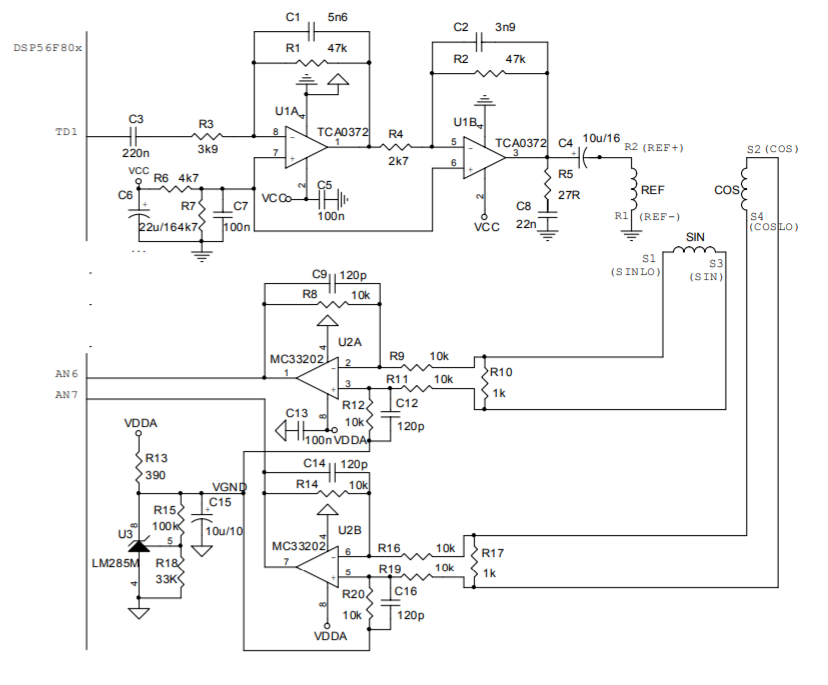
\includegraphics[width=\textwidth]{graphics/Schema_Resolver.png}
	\caption{Schema Resolver der Firma NXP.\cite{mienkina_56f80x_nodate}}
	\label{fig:Schaltung_Resolver_NXP}
\end{figure}

\paragraph{Opamp1:}\mbox{}\\

Das Dreiecksignal soll innert einer halben Periodendauer um drei Volt steigen. Das heisst, es ergibt sich gemäss Formel \ref{equ:Anstiegsrate_U1A} eine Slew-Rate von 0.048V/\textmu s.
Der auf 5.6nF dimensionierte Kondensator wird so gemässs Formel \ref{equ:Strom_C2} einen maximalen Strom von 269 \textmu A leiten. \cite{user_gast_berechnung_2009}

\begin{equation}
Slew-Rate_1 (SR_1) = \frac{\Delta_{U_1}}{T/2} = \frac{3V}{62.5 \mu s} = 0.048\frac{V}{\mu s}
\label{equ:Anstiegsrate_U1A}
\end{equation}

\begin{equation}
I_{C_2} = C_2 \cdot Slew-Rate_1 = 5.6 \cdot 10^{-9} \cdot 0.048\frac{V}{10^{-6}s} = 269\mu A
\label{equ:Strom_C2}
\end{equation}

So kann gemäss Formel \ref{equ:Dimensionierung_R1} der Widerstand R3 dimensioniert werden. Dessen Wert beträgt ungefähr 9300\textOmega. \cite{user_gast_berechnung_2009}

\begin{equation}
R3 = \frac{\pm  2.5V}{I_{C1}} = \frac{\pm 2.5V}{269 \mu A} = 9.3k\textOmega
\label{equ:Dimensionierung_R1}
\end{equation}

Mit dem Widerstand R1 und der Kapazität C2 kann die obere Grenzfrequenz bestimmt werden. Diese Grössen wurde aus dem Datenblatt des NXP-Interfaces übernommen und ergaben zusammen gmäss Formel \ref{equ:Grenzfrequenz1} eine Frequenz von:

\begin{equation}
\omega_{g1} = \frac{1}{R2 \cdot C2} = 3799 rad^{-1}
\label{equ:Grenzfrequenz1}
\end{equation}

\paragraph{Opamp2:}\mbox{}\\

Der zweite Opamp integriert das Dreiecksignal zu einem sinusförmigen Signal. Da das Ausgangssignal für die Spule 5V betragen soll und diese Änderung auch in 62.5\textmu s geschehen soll, benötigen wir eine Slew-Rate von 0.08V/\textmu s, wie mit Formel \ref{equ:Anstiegsrate_U1B} berechnet. Der daraus maximal resultierende Strom ergibt mit der in Formel \ref{equ:Strom_C3} 624 \textmu A.

\begin{equation}
Anstiegsrate_2 (SR_2) = \frac{\Delta_{U_2}}{T/2} = \frac{5V}{62.5 \mu s} = 0.08\frac{V}{\mu s}
\label{equ:Anstiegsrate_U1B}
\end{equation}

In Formel \ref{equ:Strom_C3} ist der Faktor 2 zu beachten. Dieser wird verwendet, da der Eingangsstrom dreieckförmig ist. Grundlage ist, dass die Spannung über dem Kondensator das Integral des Stromes über die Zeit ist. So ergibt sich beim Integrieren eine Fläche mit einer Spannungsamplitude von 3V mal eine Zeit von 62.6\textmu s geteilt durch 2.

\begin{equation}
I_{C_3} = C_3 \cdot Slew-Rate_2  \cdot 2= 3.9 \cdot 10^{-9} \cdot 0.080\frac{V}{10^{-6}s}  \cdot 2 = 624 \mu A
\label{equ:Strom_C3}
\end{equation}

Aus dem Maximalstrom kann der Widerstand R4 dimensioniert werden. Er beträgt ziemlich genau 2400\textOmega.

\begin{equation}
R4 = \frac{\pm 1.5V}{I_{C3}} = \frac{\pm 1.5V}{624 \mu A} = 2.4k\textOmega
\label{equ:Dimensionierung_R4}
\end{equation}

Mit dem Widerstand R2 und der Kapazität C3 kann die obere Grenzfrequenz bestimmt werden. Diese Grössen wurden aus dem Datenblatt des NXP-Interfaces übernommen und ergaben zusammen gmäss Formel \ref{equ:Grenzfrequenz2} eine Frequenz von:

\begin{equation}
\omega_{g2} = \frac{1}{R2 \cdot C3} = 5456 rad^{-1}
\label{equ:Grenzfrequenz2}
\end{equation}

\paragraph{Opamp3}\mbox{}\\

Das zurückkommende Signal muss auch gefiltert und verstärkt werden, sodass es in einem Spannungsbereich zwischen 1V und 4V liegt. Das Übersetzungsverhältnis des Resolvers beträgt 2:1, weswegen eine Spannung von \textpm \textDelta U von $\pm$ 1.25V erwartet wird. Der Differenzverstärker hat somit den Verstärkungsfaktor gemäss Formel \ref{equ:Simulation_Verstaerkungsfaktor1} von 1.2.

\begin{equation}
V = 3V/2.5V V = \frac{U_A}{U_E} = \frac{3V}{2.5V} = 1.2
\label{equ:Simulation_Verstaerkungsfaktor1}
\end{equation}

Daraus kann der Widerstand R12 berechnet werden. Dieser Beträgt gemäss Formel \ref{equ:Simulation_R12} 12k\textOmega.

\begin{equation}
R12 = V \cdot R9 = 1.2 \cdot 10k\Omega = 12k\Omega
\label{equ:Simulation_R12}
\end{equation}

Die Kondensatorgrösse wurde aus dem Datenblatt von NXP übernommen. Damit wird jedoch die Grenzfrequenz festgelegt. Diese ergibt mit R12 und C6 gemäss Formel \ref{equ:Grenzfrequenz3} 644444 rad$^{-1}$

\begin{equation}
\omega_{g2} = \frac{1}{R12 \cdot C6} = 644.44 krad^{-1}
\label{equ:Grenzfrequenz3}
\end{equation}

\subsubsection{Simulation}

Die berechneten Werte wurden in der Simulation eingesetzt. Da die Opamps und der Kondensator C1 die Schaltung beeinflussen, wurden kleine Anpassungen an den Werten von R3 und R4 gemacht, um die gewünschten Effekte zu erlangen. Die Simulationsergebnisse werden im Folgenden aufgelistet:
\begin{itemize}
\item C1 = 220nF
\item C2 = 5.6nF
\item C3 = 3.9nF
\item R1 = 9k\textOmega
\item R2 = 47k\textOmega
\item R3 = 47k\textOmega
\item R4 = 2.5k\textOmega
\end{itemize}

%Die Rück-Berechnung zur Amplitude des Ausgangssignals erhalten wir über:
%
%\begin{equation}
%I_{C1}=\frac{\pm2.5V}{R1} = \frac{\pm2.5V}{10k\Omega} = \pm 250 \mu A => \Delta_{I_{C1}} = 500\mu A
%\end{equation}
%
%mit:
%
%\begin{equation}
%Anstiegsrate = \frac{I_{C1}}{C1} = 
%\end{equation}
%
%ergibt:
%
%\begin{equation}
%\Delta U = \frac{Anstiegsrate \cdot T}{2}
%\end{equation}


%Die Spule am Referenzsignal hat einen ohmischen Widerstand von 55\textOmega, was gemäss Formel \ref{equ:Spulenstrom}zu einem Spitzenstrom von 90mA ergibt.

%\begin{equation}
%\^{I}_{Spule} = \frac{\^{U}_{Spule}}{R_{Spule}} = \frac{5V}{55\textOmega} = 0.09A = 90mA
%\label{equ:Spulenstrom}
%\end{equation}

Abbildung \ref{fig:Simulation_Referenzsignal} zeigt die Opamp-Schaltung für das Referenzsignal. Darin enthalten sind die beiden Verstärkerschaltungen in Serie geschaltet. Beide haben einen Offset von 2.5V. Der Kondensator C1 bildet einen Hochpass, woduch sich die Spannungen in der gesamten Schaltung ein wenig anheben und es eine Weile dauert, bis die Schaltung eingeschwungen ist.Die passiven Elemente R5 und C4 verhindern ein ungewolltes Schwingen des Ausgangs, wenn induktive Lasten angetrieben werden.
Abbildung \ref{fig:Simulation_Referenzsignal2} zeigt die Differenzverstärkerschaltung auf Empfängerseite.

\begin{figure}[h!]
\centering
\subcaptionbox{Schema Simulation Referenzsignal.\label{fig:Simulation_Referenzsignal}}{	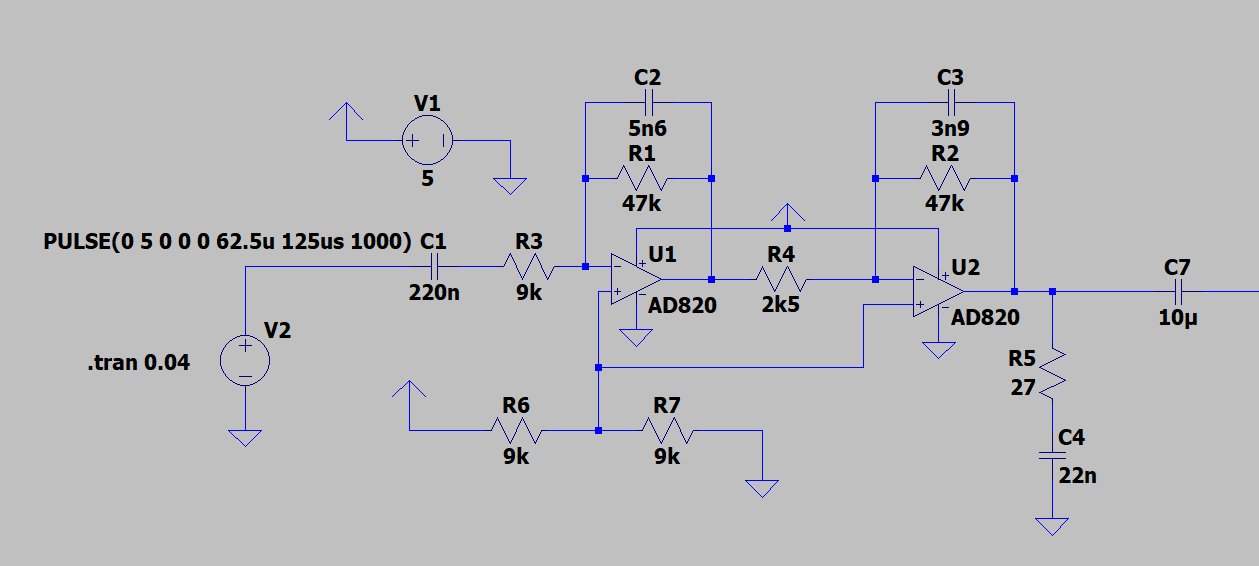
\includegraphics[height=4.5cm]{graphics/Simulation_Schema_Referenzsignal.png}}
\hfill
\subcaptionbox{Schema Simulation Referenzsignal.\label{fig:Simulation_Referenzsignal2}}{	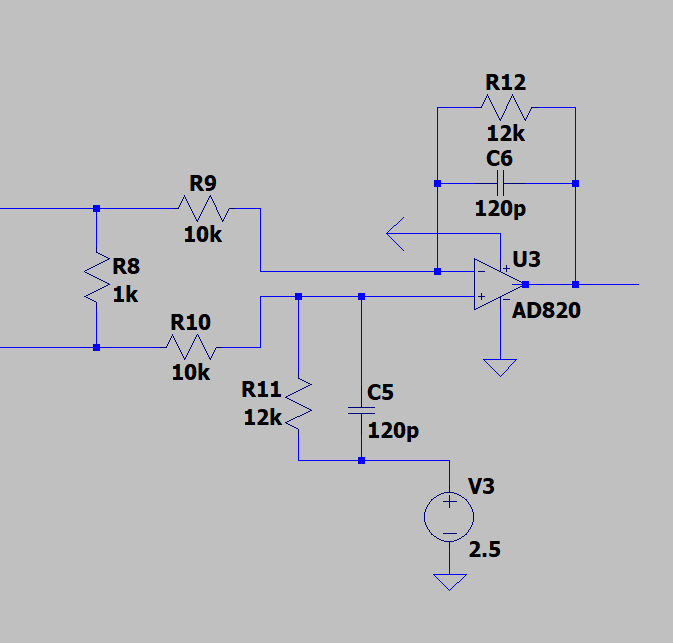
\includegraphics[height=4.5cm]{graphics/Simulation_Schema_Referenzsignal2.png}}
\hfill
\caption{Schema Simulation Referenzsignal Resolver.}
\label{fig:Simulation_Referenzsignal0}
\end{figure}

\newpage
In Abbildung \ref{fig:Simulation_Einschwingvorgang} ist der Einschwingvorgang zu erkennen. Das gesamte System ist nach etwa 20 ms eingeschwungen. Das blaue Signal ist die Spannung zwischen dm Kondensator C1 und R1, das grüne Signal ist das Dreiecksignal am Ausgang des ersten Opamps und das rote Signal ist das Sinus-Signal am Ausgang des zweiten Opamps.

\begin{figure}[h!]
	\centering
	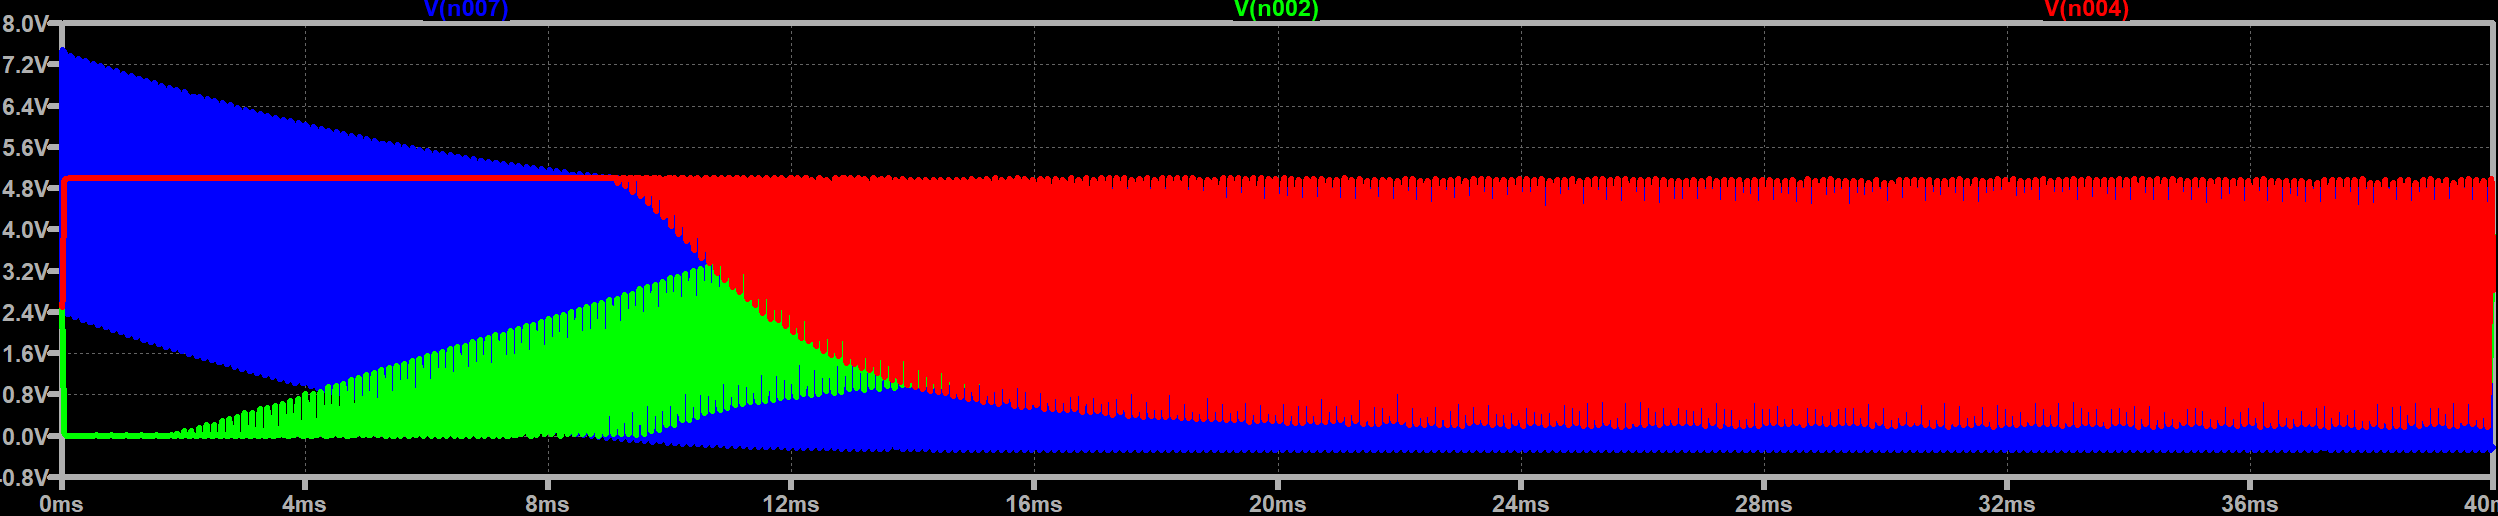
\includegraphics[width=\textwidth]{graphics/Einschwingvorgang.png}
	\caption{Einschwingvorgang}
	\label{fig:Simulation_Einschwingvorgang}
\end{figure}

%Beide Operationsverstärker werden mit Single-Supply versorgt, weshalb ein virtueller Ground erstellt wird mit den Widerständen \textbf{R704 und R706}. So Pendelt das Signal um die 2.5V Referenzspannung. Erwünscht ist ein Ausgangssignal zwischen 0 und 5 V, das heisst, dass eine Amplitude von 2.5 angestrebt wird.

%Die Schaltung wurde in LTSpice aufgebaut, um das Verhalten zu untersuchen. Folgende Resultate wurden erzielt:

%Wird nun ein Rechtecksignal eingespiesen, wird dieses Integriert. Abbildung \ref{fig:Simulation_Rechteck_Dreieck} zeigt das Rechtecksignal und das daraus resultierende Dreiecksignal.

In den Abbildungen \ref{fig:Simulation_Rechteck_Spannung} und \ref{fig:Simulation_Rechteck_Strom} ist die Spannung und der Strom am und durch den Punkt zwischen C1 und R3 zu sehen. Der Strom durch C1 und R1 ist folglich der selbe. Die Spannung an diesem Punkt ist das Eingangssignal für die Integratorschaltung am Opamp1.
\begin{figure}[h!]
	\centering
	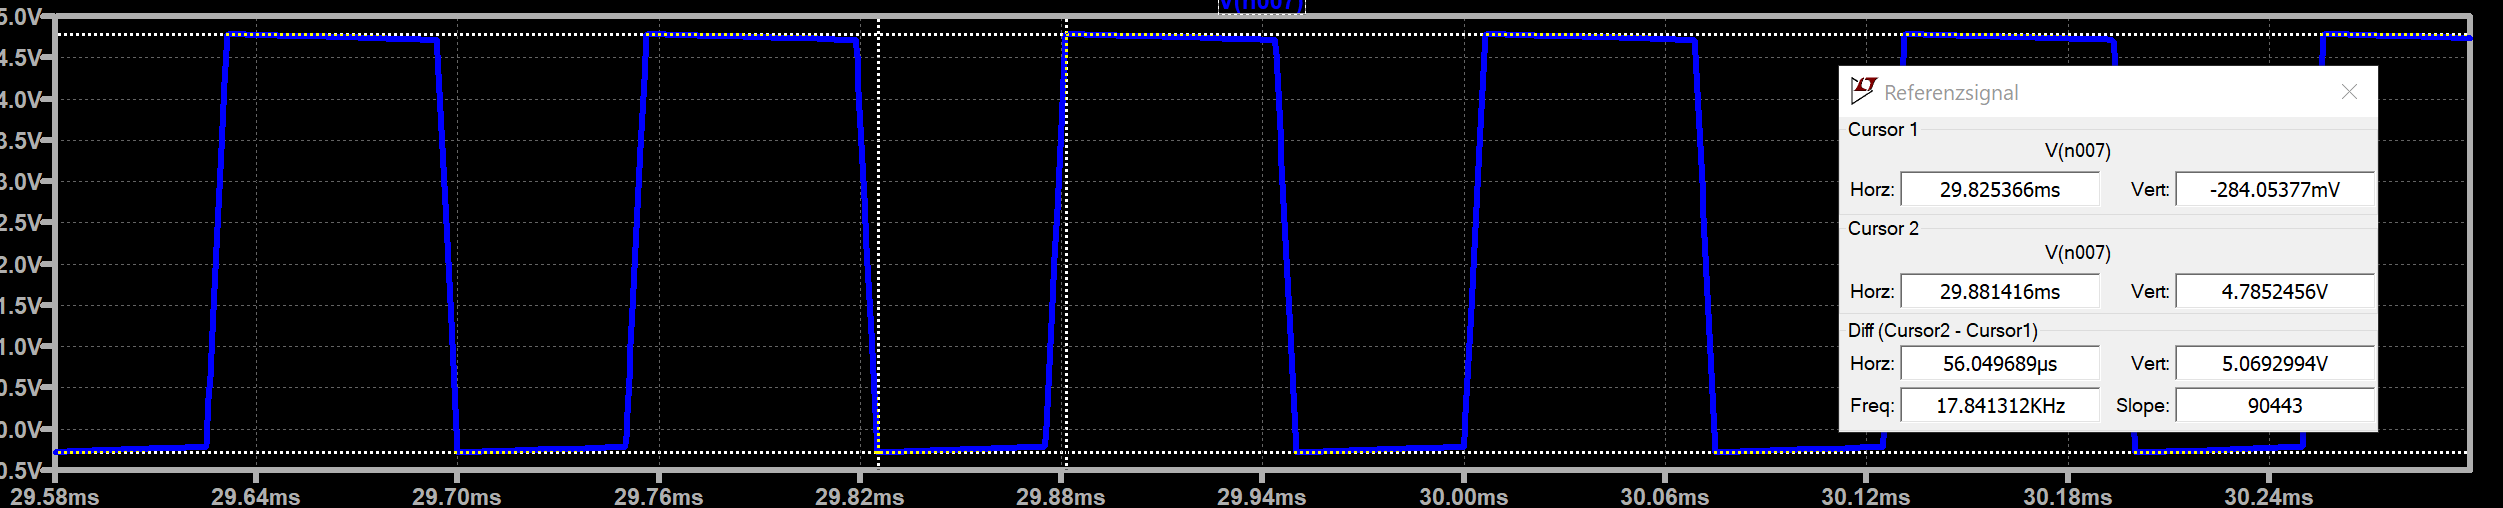
\includegraphics[width=\textwidth]{graphics/Spannung_Ue_1.png}
	\caption{Eingangs PWM-Signal zwischen C1 und R1. Zu erkennen: Durch den Strom durch R3 fällt eine Spannung über dem Widerstand ab. Der Spannungsabfall lässt sich im Rest der Schaltung nicht gross bemerken.}
	\label{fig:Simulation_Rechteck_Spannung}
\end{figure}

%
%Abbildung \ref{fig:Simulation_Dreieck_Sinus} zeigt das Sinussignal (grün), welches aus dem Dreieck generiert wurde. Sie zeigt ebenfalls das Signal, wie es aus dem Resolver zurückgegeben würde.

\begin{figure}[h!]
	\centering
	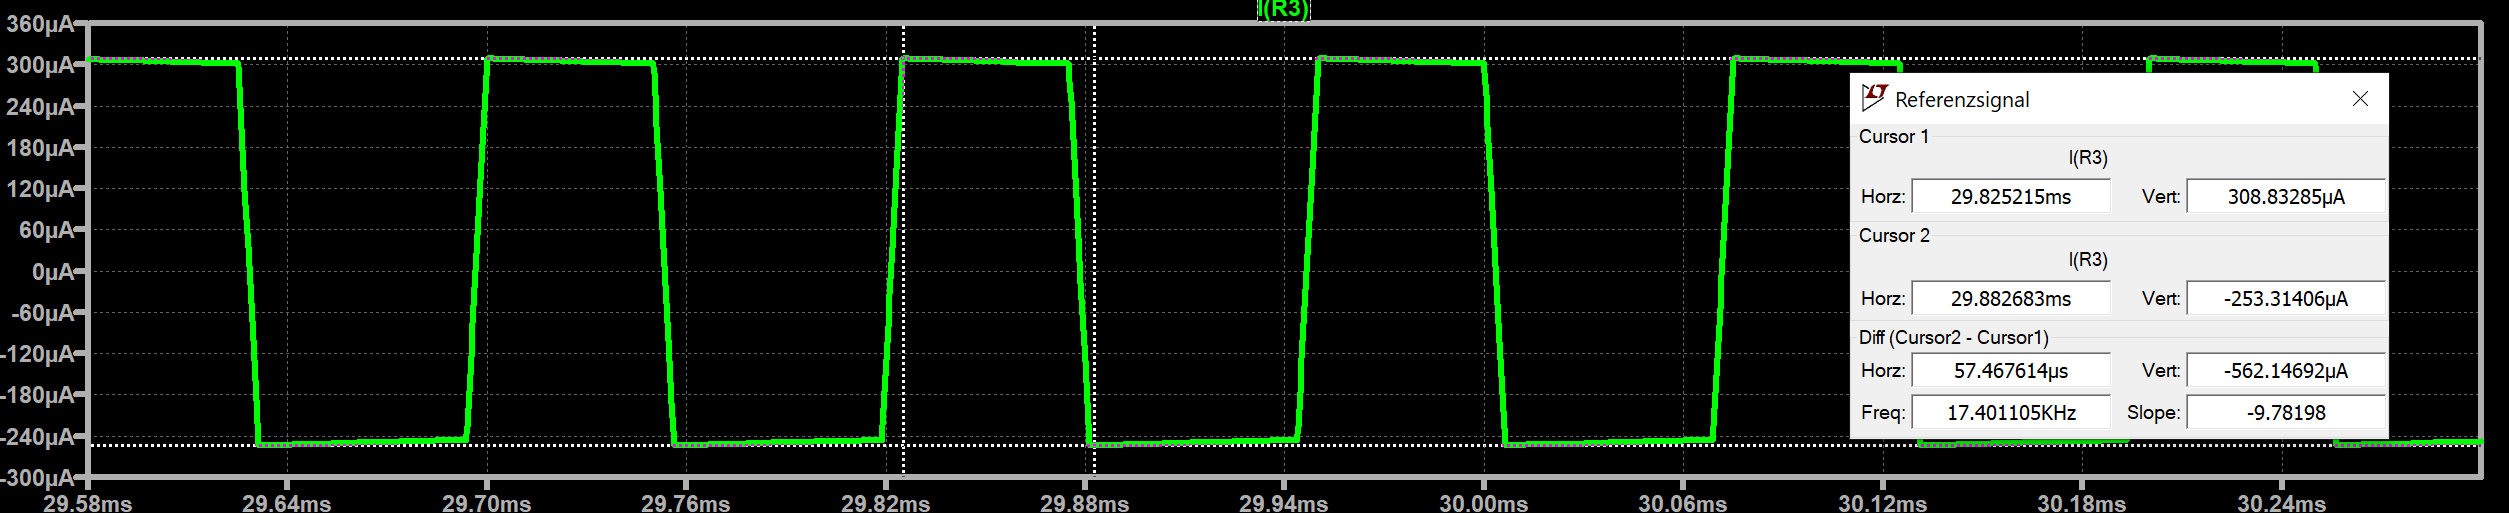
\includegraphics[width=\textwidth]{graphics/Strom_Ic1.png}
	\caption{Eingangs-Strom durch R3. Zu erkennen: Der halbe Strom I$_{P-P}$ beträgt 281\textmu A und ist somit leicht höher als in Formel \ref{equ:Strom_C2} berechnet.
	%Dies hat damit zu tun, dass der Widerstand durch Anpassungen an dessem Wert kleiner gewählt wurde. Der Strom durch den Widerstand R1 ist so klein, dass er vernachlässigt werden kann.
	}
	\label{fig:Simulation_Rechteck_Strom}
\end{figure}

\newpage

In den Abbildungen \ref{fig:Simulation_Dreieck_Spannung} und \ref{fig:Simulation_Dreieck_Strom} ist die Spannung am Ausgang vom Opamp1 und der Strom durch R4 abgebildet. Die Ausgangsspannung vom Opamp1 ist das Eingangssignal des Opamp2. 
%Die Übertragungsfunktion wurde anhand eines Bode-Plots in Abbildung \ref{fig::Simulation_Bode_1} dargestellt.

\begin{figure}[h!]
	\centering
	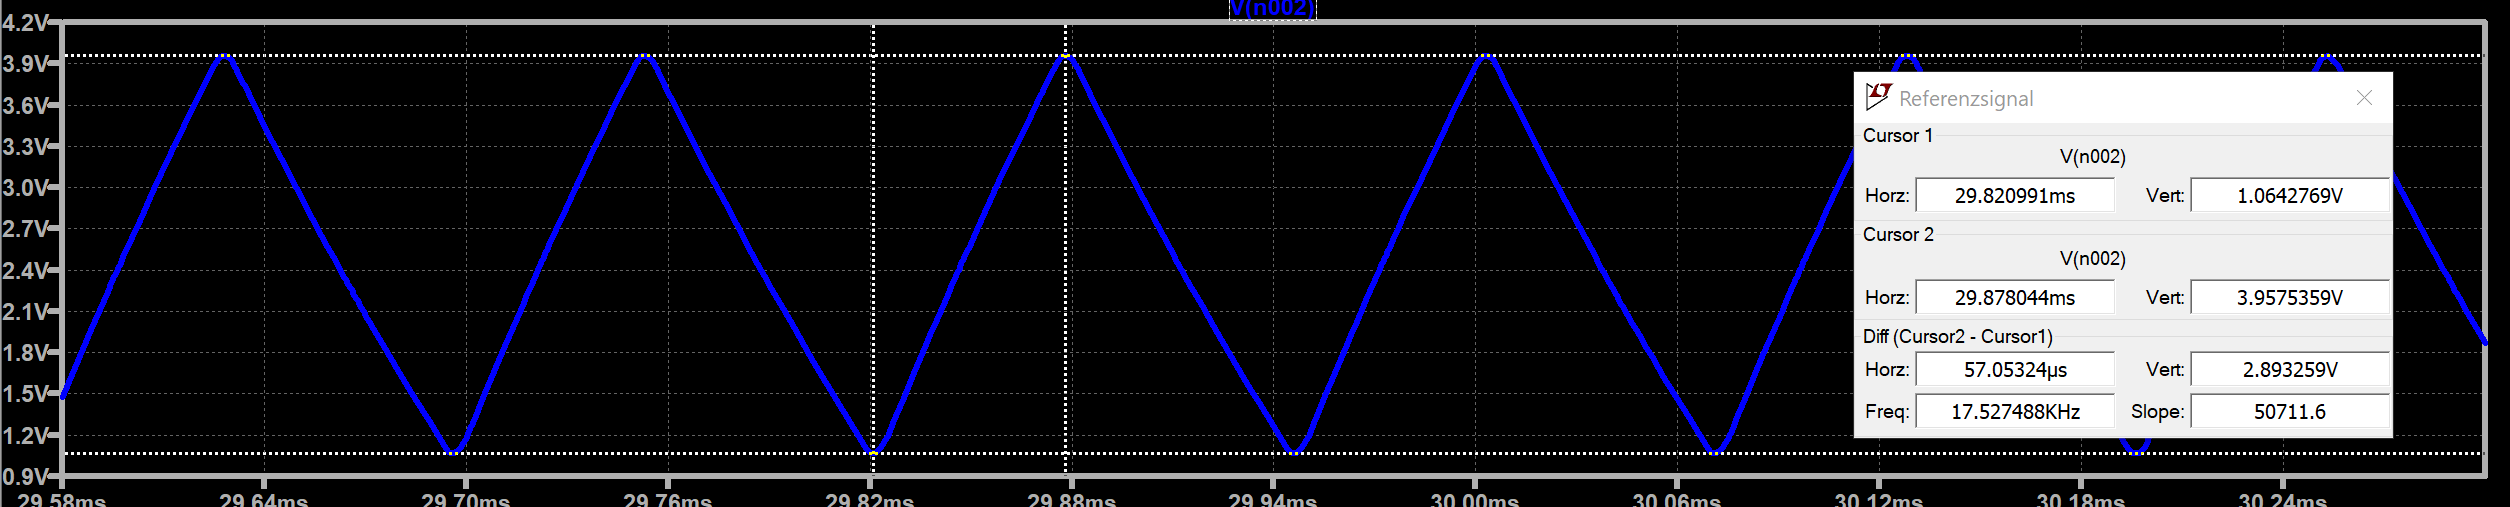
\includegraphics[width=\textwidth]{graphics/Spannung_Ua_1.png}
	\caption{Spannung am Ausgang des Opamp1. Zu erkennen: Die Peak-to-Peak-Amplitude beträgt grössenordnung 2.9V. Dies lässt sich auf die verzögerten Flanken des Opamps zurückführen, da mit einem idealen Opamp gerechnet wurde.}
	\label{fig:Simulation_Dreieck_Spannung}
\end{figure}

\begin{figure}[h!]
	\centering
	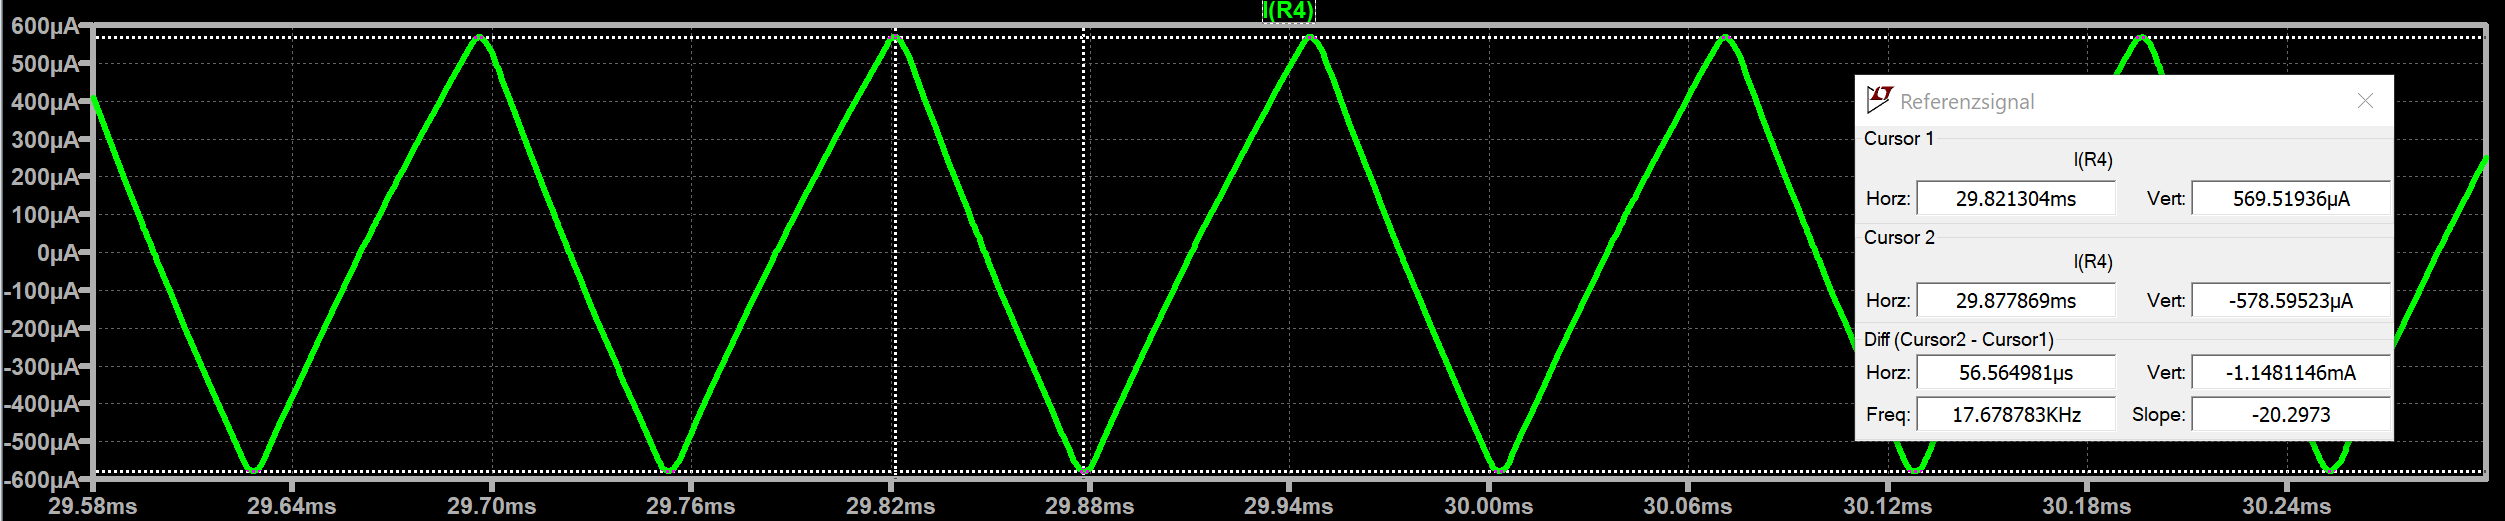
\includegraphics[width=\textwidth]{graphics/Strom_Ir_2.png}
	\caption{Eingangs-Strom durch R4. Zu erkennen: Der halbe Strom I$_{P-P}$ beträgt 574\textmu A und ist somit leicht tiefer als in Formel \ref{equ:Strom_C2} berechnet.
	%Dies hat damit zu tun, dass der Widerstand durch Anpassungen an dessem Wert grösser gewählt wurde. Der Strom durch den Widerstand R3 ist so klein, dass er vernachlässigt werden kann.
	}
	\label{fig:Simulation_Dreieck_Strom}
\end{figure}

%\begin{figure}[h!]
%	\centering
%	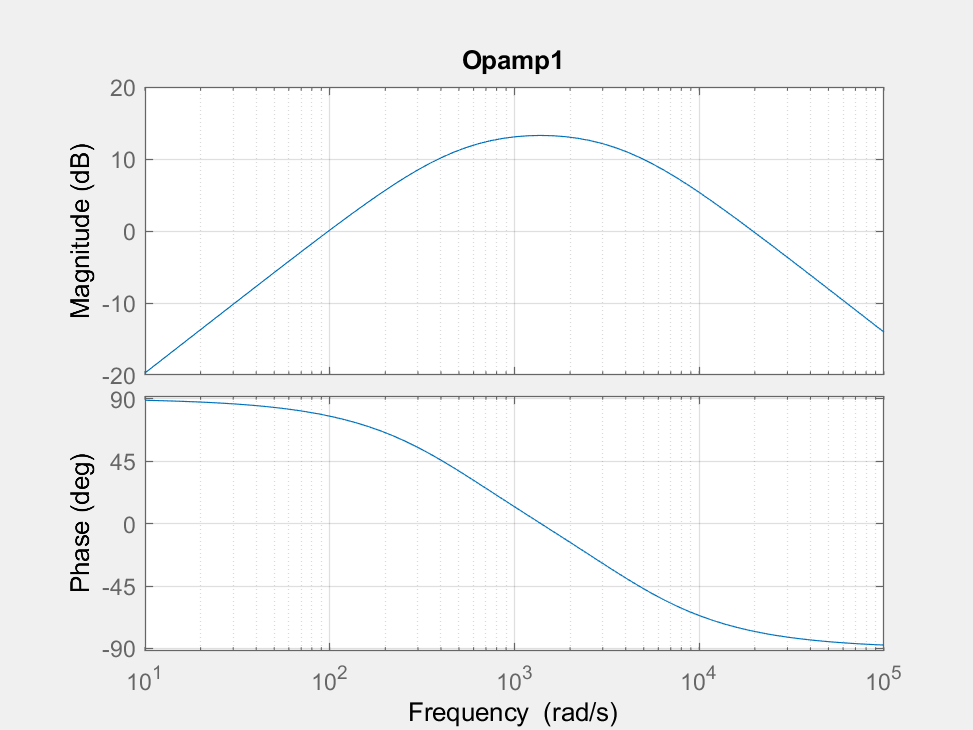
\includegraphics[width=0.5\textwidth]{graphics/Op1.png}
%	\caption{Bodeplot Übertragungsfunktion Opamp1.}
%	\label{fig:Simulation_Bode_1}
%\end{figure}

In den Abbildungen \ref{fig:Simulation_Sinus_Spannung} und \ref{fig:Simulation_Sinus_Strom} ist die Spannung am Ausgang vom Opamp1 und der Strom durch R4 abgebildet. Die Spannung am Ausgang vom Opamp1 ist das Eingangssignal des Opamp2.  
%Die Übertragungsfunktion vom Opamp2 wurde anhand eines Bode-Plots in Abbildung \ref{fig:Simulation_Bode_2} dargestellt. Die Abbildung \ref{fig:Simulation_Bode_3} zeigt die Übertragungsfunktion der beiden Operationsverstärkerschaltungen in Serie.

\begin{figure}[h!]
	\centering
	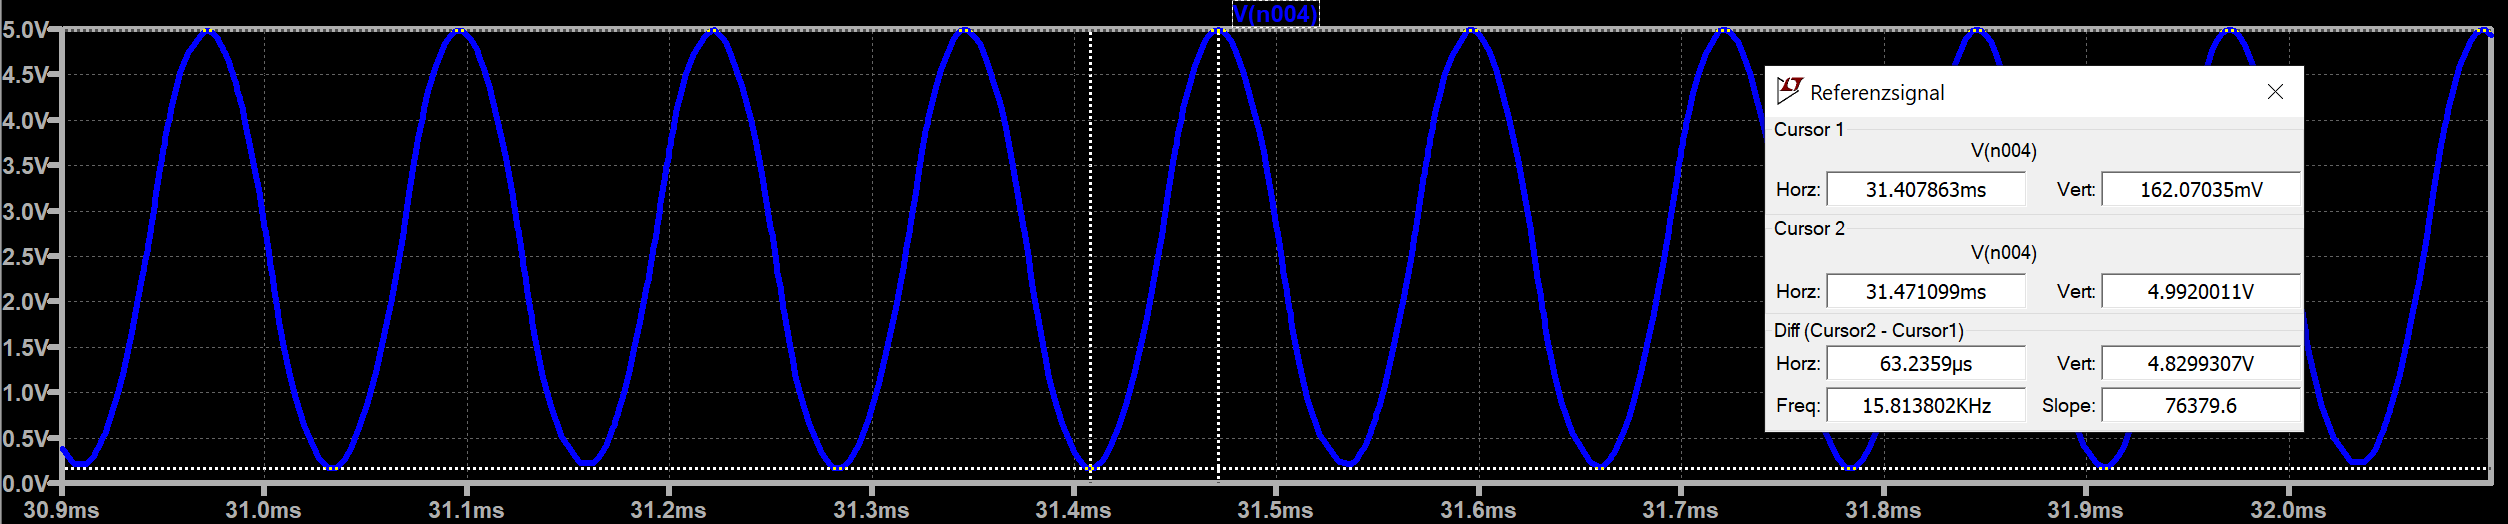
\includegraphics[width=\textwidth]{graphics/Spannung_Ua_3.png}
	\caption{Spannung am Ausgang des Opamp2. Zu erkennen: Die Peak-to-Peak-Amplitude beträgt grössenordnung 4.8V. Dies lässt sich auf die verzögerten Flanken des Opamps (idealer Opamp) und das ohnehin schon weniger starke Dreiecksignal zurückführen.}
	\label{fig:Simulation_Sinus_Spannung}
\end{figure}
\begin{figure}[h!]
	\centering
	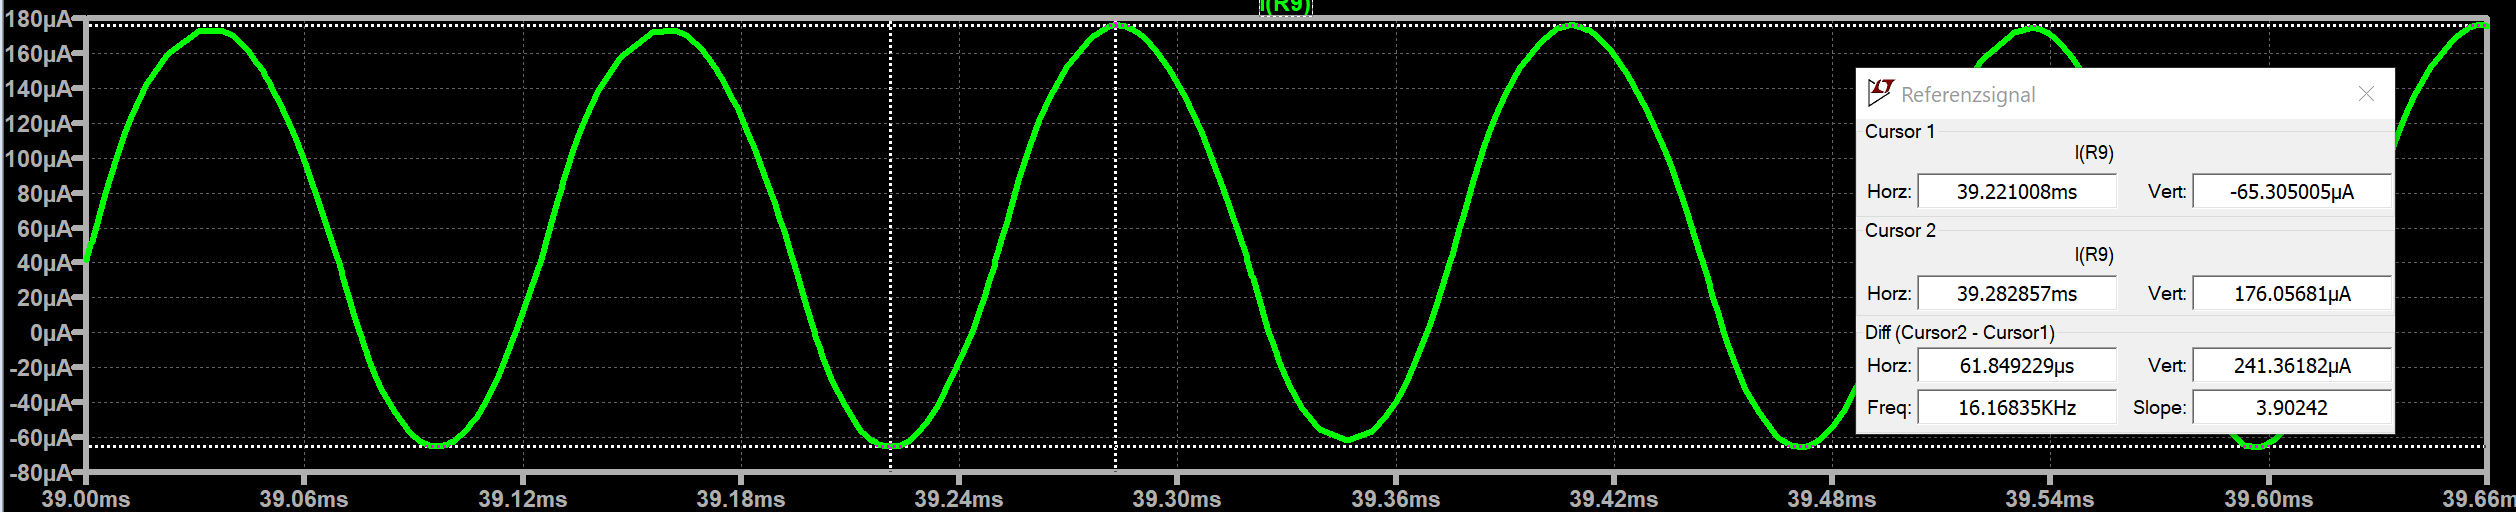
\includegraphics[width=\textwidth]{graphics/Strom_Ir_3.png}
	\caption{Strom durch R2.}
	\label{fig:Simulation_Sinus_Strom}
\end{figure}
%\begin{figure}[h!]
%	\centering
%	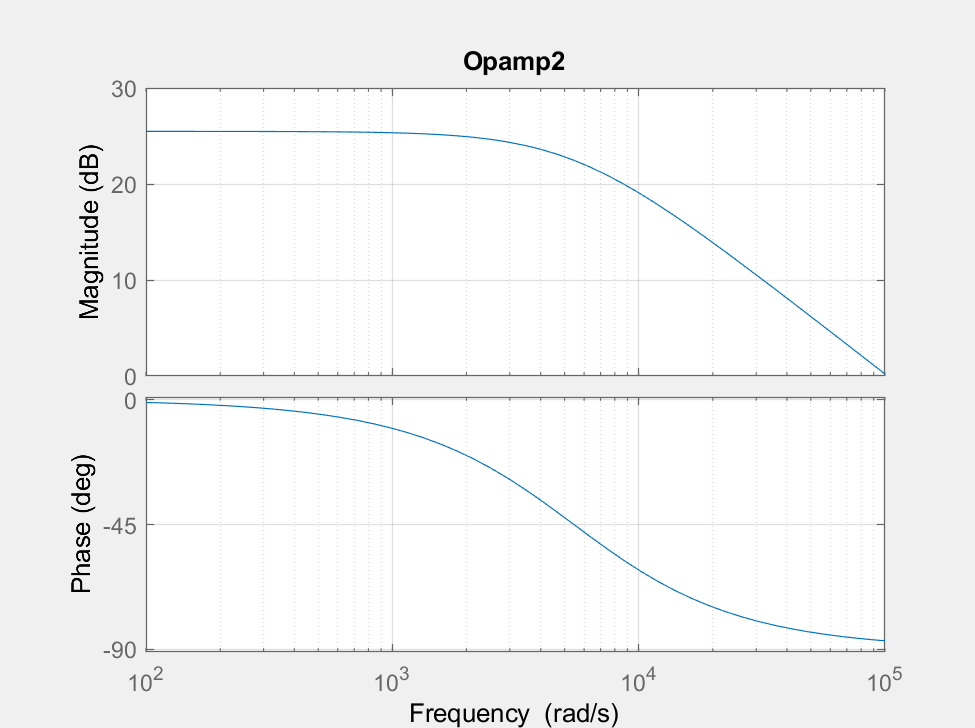
\includegraphics[width=0.5\textwidth]{graphics/Op2.png}
%	\caption{Bodeplot Übertragungsfunktion Opamp2.}
%	\label{fig:Simulation_Bode_2}
%\end{figure}

%\begin{figure}[h!]
%	\centering
%	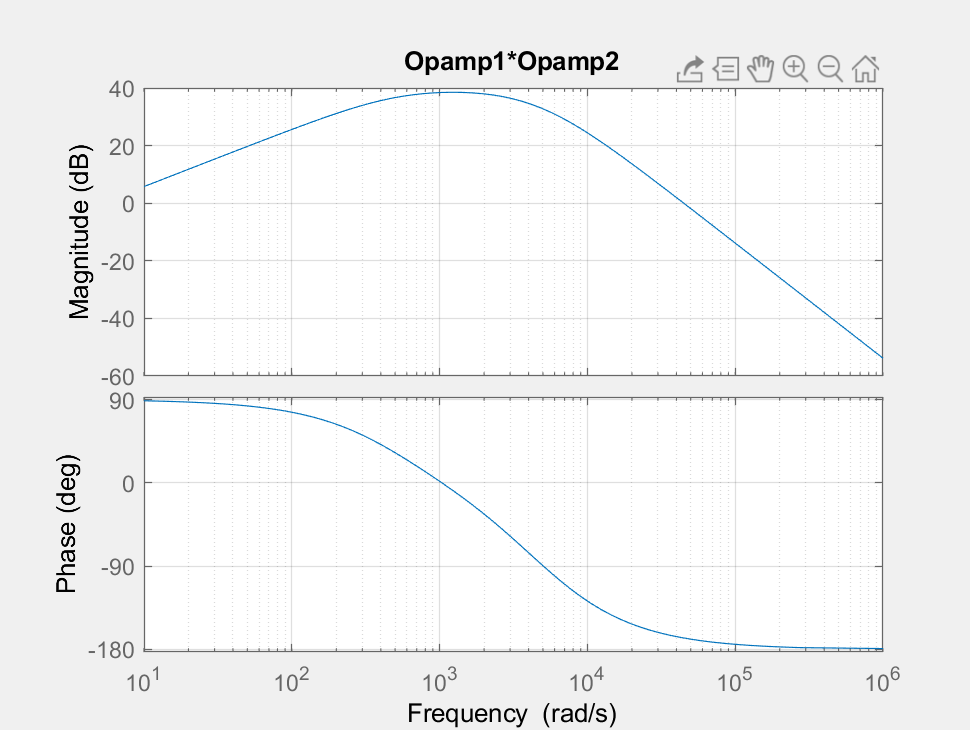
\includegraphics[width=0.5\textwidth]{graphics/Op1_Op2.png}
%	\caption{Bodeplot Übertragungsfunktion Opamp1 $\cdot$ Opamp2.}
%	\label{fig:Simulation_Bode_3}
%\end{figure}

In den Abbildungen \ref{fig:Simulation_Op3_1} und \ref{fig:Simulation_Op3_2} ist die Spannung am Ausgang vom Opamp3 und der Strom durch R9 abgebildet. Die Spannung am Ausgang vom Opamp3 ist das Eingangssignal des TMC4671. Die Ausgangsspannung für den Controller ist in Abbildung \ref{fig:Simulation_Op3_3} dargestellt.

\begin{figure}[h!]
	\centering
	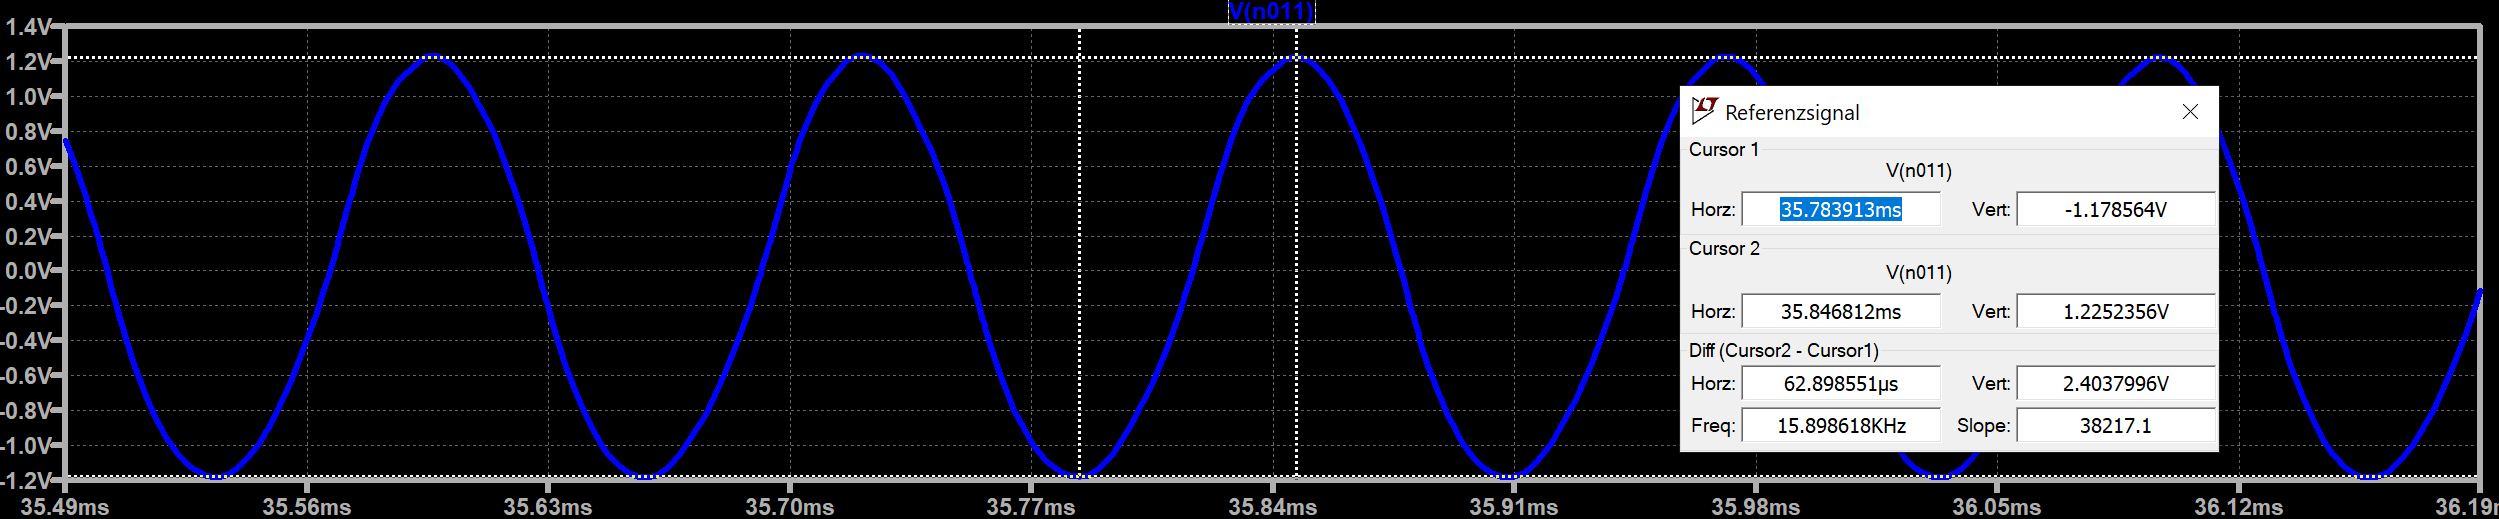
\includegraphics[width=\textwidth]{graphics/Spannung_Ue_2.png}
	\caption{Eingangsspannung für Verstärkerschaltung Mikrocontrollersignal.}
	\label{fig:Simulation_Op3_1}
\end{figure}

\begin{figure}[h!]
	\centering
	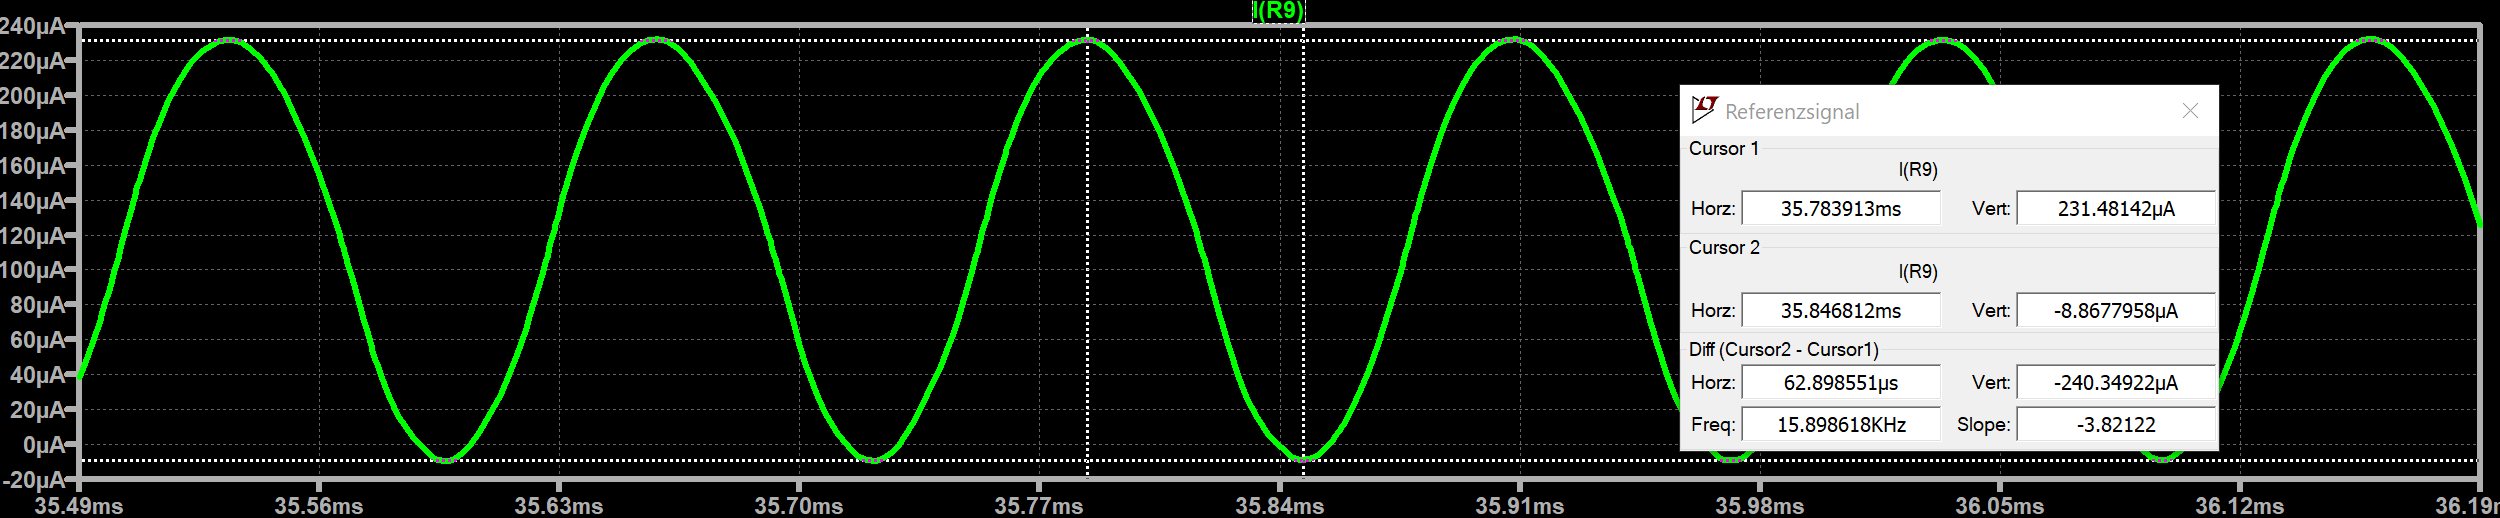
\includegraphics[width=\textwidth]{graphics/Strom_Ir_4.png}
	\caption{Strom durch Widerstand R9.}
	\label{fig:Simulation_Op3_2}
\end{figure}

\begin{figure}[h!]
	\centering
	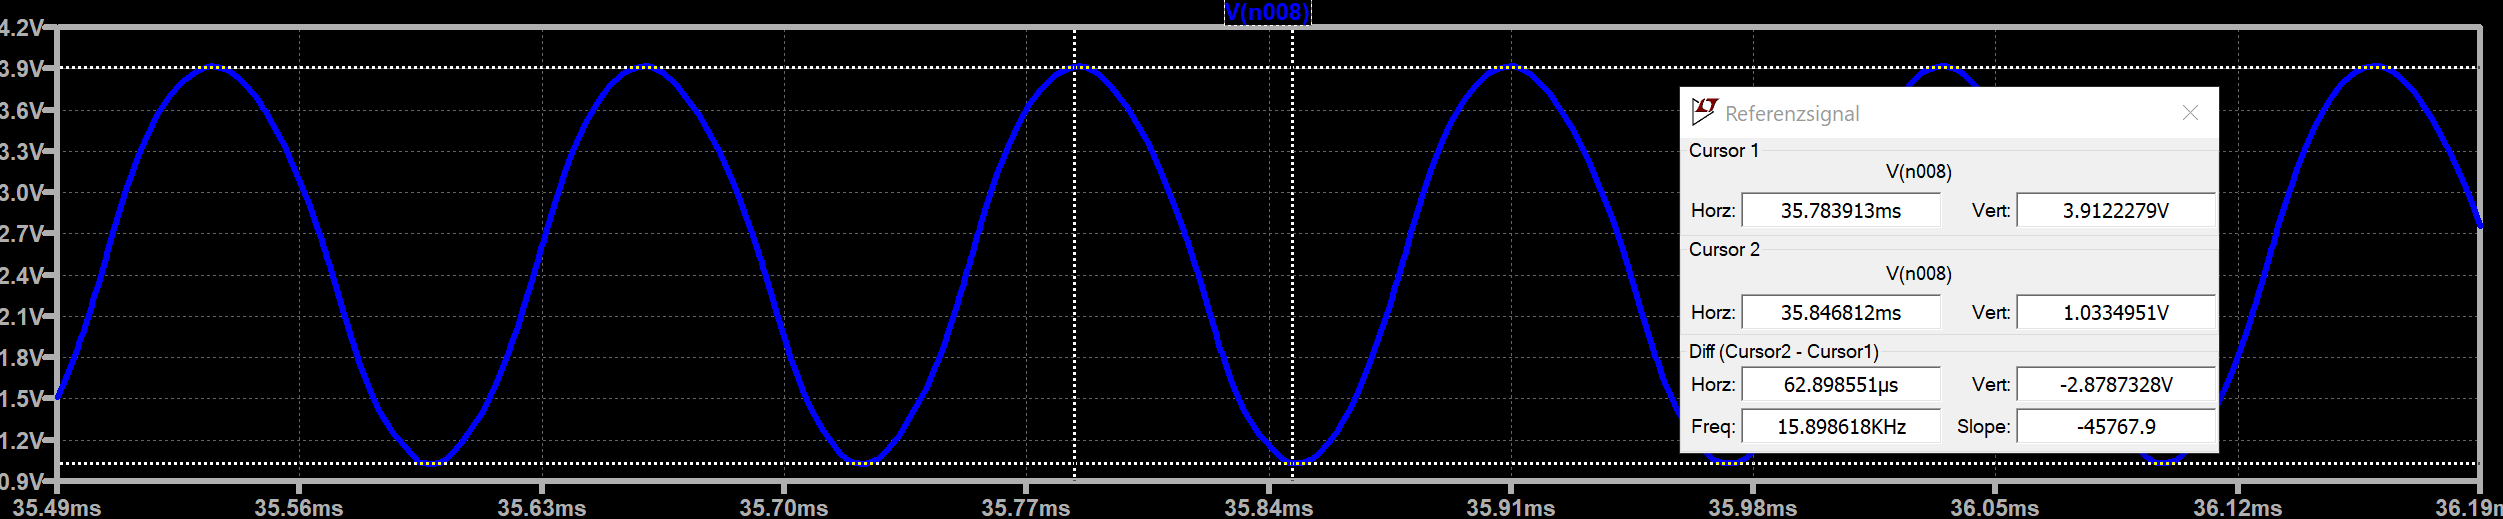
\includegraphics[width=\textwidth]{graphics/Spannung_Ua_4.png}
	\caption{Ausgangsspannung für TMC4671. Zu erkennen: Das Signal liegt zwischen 1V und 4V, wie es der Controller braucht.}
	\label{fig:Simulation_Op3_3}
\end{figure}

%\begin{figure}[h!]
%	\centering
%	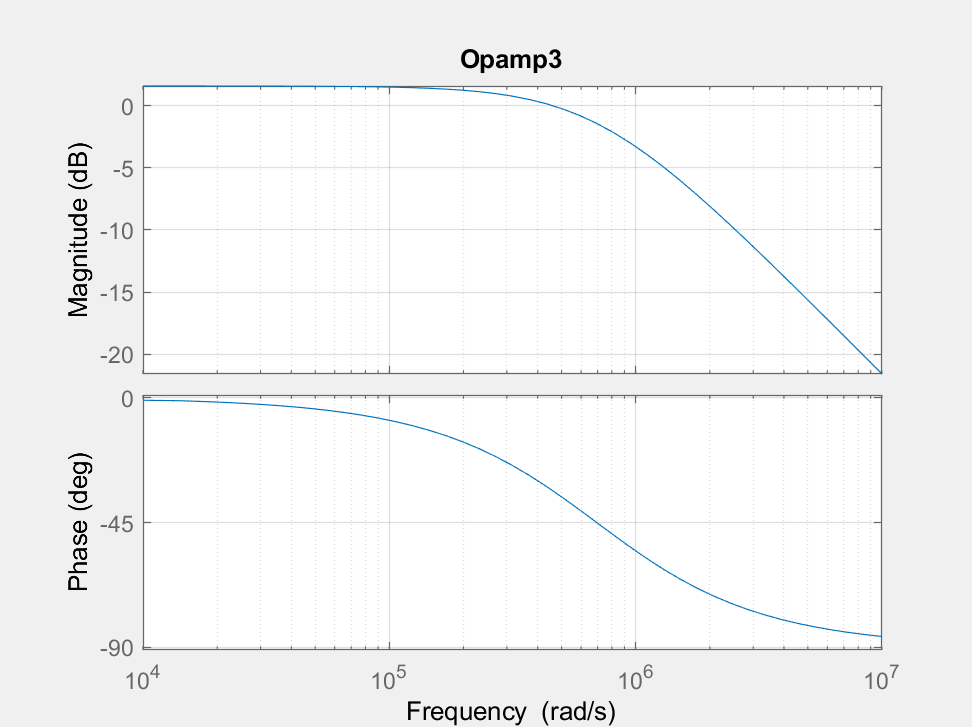
\includegraphics[width=0.5\textwidth]{graphics/Op3.png}
%	\caption{Bodeplot Übertragungsfunktion Opamp3.}
%	\label{fig:Simulation_Bode_4}
%\end{figure}